\chapter{Introduction}

A computer's processor is an amazing device: it executes millions of operations each second, at a speed difficult to grasp for any human. Still, these operations are performed on simple and precise data types: read 32 bits from memory address X into register R1, subtract R1 from R2 using unsigned 32-bit integer semantics, etc. For the processor, data is made up of bits and each operation needs to know the exact size and semantics of its operands, since this ultimately dictates which bitwise operations have to be executed.

On the completely opposite side of the spectrum, people think in terms of very high-level goals, such as the desire to find the 10th or 100th Fibonacci number. There's no mention of the exact number of bits used to represent the number and, from the context, it's clear the numbers must be positive. Programming languages and compilers bridge the gap between high-level goals and the precise low-level machine instructions necessary to implement them: Programming languages allow people to express their intent while compilers translate this intent, written in the source code, to precise low-level machine instructions.

Programming languages have long struggled with a dilemma: exposing low-level data types and their operations allows precise control and a very direct translation to machine code, but also reduces the programmer productivity. Indeed, programming languages such as Assembly and C allow very precise control over all aspects of the computation and the interaction between the processor and the other devices in the computer. Yet this forces the programmer to make many decisions that are not directly related to the problem: how to store data, how each operation manipulates it and what needs to be done at each step. In fact, this very tight control over the execution, exposing all the possibilities and asking the programmer to make all the decisions slows down  development and makes it more error-prone.

The other alternative is exposing high-level data types and operations in the programming language. For example, languages such as Scala, Python, Ruby and JavaScript gloss over many implementation details to offer a high-level environment that boosts the programmer productivity. For example, Python automatically adjusts the bit width of integer numbers so operations never overflow, thus completely eliminating the choice of size and protecting the programmer from the risk of overflows. Similarly, the Scala standard library offers data structures such as arrays, vectors, lists that can hold any kind of values, be it integers, floating-point numbers, database records or objects representing other nested data structures. In doing so, the language relieves the programmer from the burden of deciding how many bits to store in each cell or what to do about nested variably-sized data structures.

But flexibility comes at a high price: high-level constructs are compiled to long sequences of machine instructions, where most of the data stored inside heap-allocated objects and operations are executed through indirect calls. Therefore, using very high-level constructs that adapt to many different use cases can incur significant slowdowns compared to their low-level equivalents, which only handle one case. For example, iterating over an array of sensor reading objects can be up to 5$\times$ slower than iterating over a hand-written data structure where each component of the reading is stored directly in its own array.

Much of the flexibility provided at the language level remains unused in real programs. For example, in practice, it is rather uncommon for a program to store both integers and strings in the same list. But, if the language allows it, the low-level code must be prepared to handle any mix of values, which makes it complex and inefficient. Yet, there is a category of programming languages where the compiler knows the type of all elements in a list: statically typed programming languages. In these languages, the static type information can guarantee that a list will only store 32-bit integers throughout its lifetime. From there, a natural question to ask is whether we can devise a more efficient version of the list for 32-bit integers and automatically use it in the program? Or, given a program written with variable-width integers, but which in practice only uses 16-bit integers, can the compiler automatically use a more efficient data representation and thus improve the execution performance?

This is where this thesis makes its main research contribution: it describes Late Data Layout, a general mechanism that allows compilers to use type information to safely replace the data representation used in a program without affecting its semantics. We markedly allow the data representation definition to be vague, since the mechanism adapts to anything from primitive numeric types to replacing complex data structures, such as arrays of sensor readings, by more efficient equivalents. All the examples we mentioned so far are automated using our mechanism and are thoroughly described in the thesis, complete with the evaluation details. % Transforming the data representation for these examples yields speedups of up to 8$\times$, but the thesis describes other examples where the improvements are even more significant.

% The two key features of this mechanism, which we call Late Data Layout, are: (1) its first-class support for object-oriented patterns, such as dynamic dispatch, method overriding and class inheritance and (2) its coherent and predictable nature, compared to the most common compiler optimizations, which may or may not kick in based on predefined heuristics. Furthermore, the program transformations we have developed using this mechanism show it is general enough to accommodate many different optimizations: from improving generics, avoiding heap allocation and all the way to allowing programmers to fine-tune their data structures after the fact. The next section gives a rough sketch of the transformations that motivated the Late Data Layout mechanism and its main features.

Although the main research contribution is the Late Data Layout mechanism, the technical artifact of the thesis is a generics compilation scheme called miniboxing (Chapter \ref{chapter:miniboxing}), which improves the performance by factors ranging from 1.1$\times$ all the way to 20$\times$. Miniboxing has motivated the development of the Late Data Layout mechanism (Chapter \ref{chapter:ldl}) and its extension (Chapter \ref{chapter:ildl}), both of which ultimately served as building blocks used in the generics transformation (Chapter \ref{chapter:mbox2}). The next section gives an overview of each chapter and explains how the work evolved motivated by the needs of the miniboxing transformation.

% Story of development:
%  1. miniboxing
%  2. LDL
%  3. iLDL
\section{Thesis Outline}

Throughout the thesis, several parts of the data representation transformation puzzle are explained. The common theme is the miniboxing transformation, which improves the performance of Scala generics running on the Java Virtual Machine environment. This section explains how the different chapters of the thesis work together to implement different aspects of the miniboxing transformation.

% The miniboxing generics compilation scheme is the running thread throughout the thesis.
% The Late Data Layout (LDL) mechanism was developed in the context of the Scala programming language, which is compiled to Java Virtual Machine bytecode.
%
% In fact, the work on LDL was motivated by the miniboxing generics transformation, which improves the performance of Scala generics and which required a complex representation transformation to be applied necessary for miniboxing was complex enough that it mandated the development of LDL. In this section we show the timeline of this development, explaining the motivation behind LDL and its main properties.

\subsection{The Miniboxing Data Representation (Chapter \ref{chapter:miniboxing})}

\begin{wrapfigure}{r}{50mm}
  \centering
  \vspace{-3em}
  \includegraphics[width=50mm]{mbox2-white.pdf}
  \vspace{-3em}
  \caption{Miniboxing Logo}
\end{wrapfigure}

% Generics in the Scala programming language => erasure => boxing
Genericity, also known as parametric polymorphism in functional languages, is a very powerful tool for abstraction: in a statically typed language, it allows defining data structures and algorithms that operate identically for different types of data. For example, the standard linked list class in the Scala library is parameterized on type of its elements: |List[T]| signals the type of elements is |T|. Still, regardless of the instantiation of |T|, the list preserves the same contract and asymptotic behavior for all its operations. This increases both safety, as the elements are statically guaranteed to be of type |T| and code reuse, since the same class can be employed in different contexts: programmers can create lists of 32-bit integers, floating point numbers, strings or any other nested objects or data structures.

However, under the hood, the Java Virtual Machine (JVM) execution platform only supports defining non-generic (monomorphic) classes. Therefore, the generic information in the programming language must somehow be projected onto the more restrictive bytecode, producing monomorphic classes. The default solution taken by both the Java and Scala compilers is to use a transformation called erasure \cite{java-erasure}, which compiles a generic class to a single bytecode entity: a monomorphic class where the type parameters are erased to their upper bounds. The upper bound of a type parameter is the most specific type known to be a subtype of our type parameter. For example, when we write |<T extends Serializable>|, the upper bound is |Serializable|, since any instantiation of the type parameter must also be a subtype of |Serializable|. By default, defining a type parameter without bounds results in the upper bound being |Object|, the top of the Java type system.

But there is a problem: references to the type parameter |T| are erased to |Object| or to more specific subtypes, but primitive types are not subtypes of |Object|. This prevents primitive data types from being stored directly in a generic collection, such as a linked list. Fundamentally, there is a tension between the different sizes and semantics of the incoming data and the fact that there is a single class which must handle everything. The technical solution taken is to encode primitive types, such as booleans, bytes, integers and floating-point numbers into heap objects, so they can be handled similarly to strings, data structures and other programmer-defined objects. Yet, this operation, known as boxing, is inefficient, introducing indirections and inefficiencies and inflating heap requirements.

% Specialization in Scala => too much bytecode
The first solution to improve generics in Scala was implemented in 2009 by \textem{Iulian Dragos} \cite{iuli-thesis, specialization-iuli}: instead of compiling the list into a single bytecode class, specialization would create multiple variants, each adapted for a primitive type. Specifically, of the ten variants, eight were adapted for the primitive types in Java, one was adapted for |Unit|, which is the Scala equivalent of Java's |void| and one was compiled with erasure, so it would hold heap-based objects. For a class like |Tuple2|, which has two type parameters, specialization would create $100$ versions, corresponding to the Cartesian product of the ten variants for each type parameter. Furthermore, since specialization is a compile-time transformation, all of the variants become part of the compiled bytecode. This prevents specialization from being used extensively throughout the Scala library, where many classes have two or even three type parameters, since it would generate impractical amounts of bytecode.

% Miniboxing => encode everything as a primitive
We begin this thesis where specialization left off: addressing the large number of specialized variants generated when compiling generic classes. In miniboxing, we propose using 64-bit long integers to encode the primitive values\footnote{We extend the term ``value'' to mean either a final variable (``value'' in the Scala vocabulary), a variable, an argument or the return of a method. This notation is used consistently throughout the thesis. For immediate constants such as the integer 5 we use the term ``constant'' or ``constant value''.}. Using the miniboxed data representation, instead of generating ten variants per type parameter, we only generate two\footnote{In the latest implementation of the miniboxing compiler plugin, version 0.4, the miniboxing transformation generates three variants instead of two, in order to avoid negative interactions with the HotSpot Just-in-time compiler in the Oracle Java Virtual Machine. More information is available on the miniboxing plugin website \cite{miniboxing-www}.}, reducing the amount of bytecode. Yet, the transformation is more complex than specialization and has many interesting interactions with the rest of the language, all presented in Chapters \ref{chapter:miniboxing} and \ref{chapter:mbox2}.

% But then T, the type parameter, can be represented as long integers in the ... => LDL
The problem that motivated the creation of the Late Data Layout mechanism was that, in the miniboxing-specialized variant of a generic class, type parameters would be stored as long integers. Unlike the typical allocation sinking compiler optimization, in our case the transformation had to be done in a predictable manner, where a certain values would be transformed regardless of whether they escape or not. Furthermore, the transformation would have to be undone in some cases, to preserve language features such as dynamic dispatch (e.g. calling the |toString| method on a value of type |T|) and subtyping (e.g. assigning a value of type |T| to a supertype).

The for the initial prototype of miniboxing, the transformation from |T| to |long| in the miniboxed variant of a class was done using the simple and conservative syntax-based transformation described in \ref{mbox:sec-mb-traf}. But the problems in scaling this transformation to all the source code patterns expressible in Scala created a need for a better, more principled transformation mechanism. This is how Late Data Layout came to be.

\newpage

% Inspired by the Scala erasure transformation itself, which unboxes scala.Int into the 32-bit ...
\subsection{Late Data Layout (Chapter \ref{chapter:ldl})}

\begin{wrapfigure}{r}{40mm}
  \centering
  \vspace{-2em}
  \includegraphics[width=40mm]{ldl-frog.pdf}
  \vspace{-1em}
  \caption{LDL Logo}
  \vspace{-2em}
\end{wrapfigure}

The Late Data Layout mechanism was developed to consistently and optimally transform the data representation inside miniboxed code. Specifically, miniboxed variants should represent values of type |T| as 64-bit long integers whenever possible. Certain code patterns, such as dynamic dispatch, assigning miniboxed values to supertypes and interacting with erased generics, require the values in their object-based representation. Additionally, in some cases, values have to remain in their object-based representation to preserve the overriding relation between methods. To implement all these requirements, LDL allows selecting the representation of each value individually.

The LDL mechanism generalizes the transformations performed in the Scala compiler backend to implement |scala.Int|. In Scala, |scala.Int| is a built-in type that represents a 32-bit integer but abstracts over the boxed and unboxed representations. This saves programmers the trouble of deciding the exact representation to use. In the compiler backend, |scala.Int| is transformed to either an unboxed integer (|int| in Java and JVM bytecode) or to a boxed one (|java.lang.Integer|) and conversions between the two representations are introduced as necessary. % We were inspired by this transformation, which is done during the erasure phase in the Scala compiler, to design LDL.

% Yet, to for the design of LDL, we made several choices that make it suitable for miniboxing: LDL is selective in the choice of data representation, consistent in its treatment of representations and optimal in terms of the number of coercions executed at runtime.

Both miniboxing and unboxing primitive types share a common trait: there is a high-level type (the type parameter |T| or |scala.Int|) that can be represented in two\footnote{Or more, the LDL mechanism does not limit the number of representations.} ways, one more efficient and the other more flexible. As the compiler transforms the high-level type into its representations, it also introduces conversions in order to keep the overall consistently of the program. Additionally to what the Scala backend does, the LDL mechanism allows selectively picking the representation of each value, a property we exploit heavily in the miniboxing transformation.

Without going into the implementation details, there are three properties of LDL that result from its current design:

\begin{itemize}
  \item Selectivity in the choice of data representation, at the level of individual value;
  \item Consistency in terms of passing values between representations; % transformation is provably correct;
  \item Optimality in terms of the number of coercions executed at runtime\footnote{Currently a conjecture, we are working on a formal proof.}.
\end{itemize}

% An important insight in LDL is that type annotations are a perfect vehicle for carrying representation information.  To start the transformation, values have their types annotated with the target representation. At the beginning, annotated and non-annotated types are compatible, allowing the abstract syntax tree (AST) rewrites to go through without regard for the final representation of each individual value. This is when the miniboxing transformation creates the specialized variant of the list, meant to store primitives and uses it in the program code to replace the erased list where possible.
%
% Once all representation-agnostic transformations were performed, the next phase in the LDL mechanism differentiates between annotated and non-annotated types, requiring conversions (also called coercions) to be inserted when the data representation changes. This phase allows LDL to automatically insert coercions where necessary, such as, for example, when using an encoded value (long integer) as the receiver of a method call, such as |toString|. Finally, after the coercions have been added to the

Miniboxing makes full use of the three properties, allowing it to completely offset the code transformation to LDL and focus on the other usability aspects. LDL scales not only to miniboxing and unboxing Scala primitive types, but also to implementing value class inlining \cite{gosling-value-classes,rose-value-classes-tearing,rose-value-classes-vm} and compiler support for multi-stage programming \cite{tiark-lms, scala-virtualized}. While further developing the miniboxing compiler plugin, we realized there were other transformations necessary to efficiently support the functional aspects of the Scala language, which led to the development of data-centric metaprogramming.

\subsection{Data-Centric Metaprogramming (Chapter \ref{chapter:ildl})}

\begin{wrapfigure}{r}{40mm}
  \centering
  \vspace{-2em}
  \includegraphics[width=40mm]{ildl-frog3.pdf}
  \vspace{-1em}
  \caption{Data-Centric Metaprogramming Logo}
  \vspace{-2em}
\end{wrapfigure}


Data-centric Metaprogramming is an extension of LDL that makes data representation transformations accessible to programmers. Through entities called transformation description objects, programmers can target values of specific types and safely replace their data representations by custom, more efficient alternatives. Any type in the language can be targeted, from simple classes all the way to generic data structures. The alternative representation is written by the programmer, and it can be based on run-time profiling information or knowledge of how the data is used. Then, once the transformation has been defined, to trigger it,  programmers enclose anything from expressions to entire class definitions inside transformation scopes, where the compiler automatically uses the custom, improved representation.

% Example:
There are many examples of using data-centric metaprogramming to improve performance:
\begin{itemize}
  \item Splitting arrays of records into records of arrays, to improve locality;
  \item Transforming eager collections in a scope into more efficient lazy collections;
  \item Replacing variable-width integers by more efficient fixed-width integers in predefined scopes where numbers are known to fit;
  \item Specializing a class from a library, which previously was impossible without changing the class source code.
\end{itemize}

Of course, programmers still have the possibility to refactor their code by hand instead of using data-centric metaprogramming. Yet, the cost of doing so in large code bases quickly becomes prohibitive and, lacking clear benchmarks, there is no guarantee the refactoring would pay off. Instead, data-centric metaprogramming allows writing idiomatic code which is automatically improved by the compiler, based on the transformation definitions.

% metaprogramming
What makes this extension unique is that it allows programmers to improve the data representation based on their own usage patterns, instead of limiting them to a fixed set of predefined compiler optimizations. This custom nature brings our approach close to metaprogramming. Yet, unlike metaprogramming, where the abstract syntax trees representing the program can be manipulated directly, potentially breaking semantics, data-centric metaprogramming only allows a limited and well-behaved set of transformations that offer correctness guarantees in terms of preserving the object-oriented aspects of the language.

% + extended LDL with additional support for custom bypass methods and bridge method support
% The data-centric metaprogramming support in the Scala compiler is added using an LDL-based compiler plugin. This extends LDL in three important ways:
%
% \begin{itemize}
%   \item[(1)] It allows users to define the transformations themselves;
%   \item[(2)] Transformations can be safely limited to scopes;
%   \item[(3)] Despite the scoped nature, the transformation is extended to correctly preserve the object-oriented model despite potential signature transformations.
% \end{itemize}
%
% The scoped nature of the data-centric metaprogramming approach was then used in miniboxing to make functional aspects of the Scala programming language more efficient.

\subsection{Scaling Miniboxing To Scala (Chapter \ref{chapter:mbox2})}

The last chapter of the thesis presents the technical challenges of scaling the miniboxing transformation to the entire Scala language, with problems such as interoperating with erased and specialized generics and efficient construction and access for core language constructs, such as tuples, functions, arrays and type classes.

In particular, the most interesting part is how a scoped transformation is used to introduce a more efficient function encoding, which allows miniboxed code to efficiently call Scala functions, which use the older specialization compilation scheme. The function transformation was initially implemented in the miniboxing plugin but we later separated it into the data-centric metaprogramming project. This shows how the three projects have been developed together throughout their existence, with the miniboxing plugin being the technical artifact and Late Data Layout being the underlying transformation.

The next section describes the context of the work and its goals (and non-goals).

\section{Context and Goals}

This section describes the context of the work, motivating the key design decisions in the miniboxing and data-centric metaprogramming projects. The choices in the late data layout mechanism are mostly a consequence of the key decisions in the other projects and the context of the work.

\subsection{Implicit Representation Choice}

The first design goal in both the miniboxing and data-centric metaprogramming projects is to avoid directly exposing representations to the programmer, instead only offering a high-level type. This stems from the desire to reduce the number of decisions a programmer needs to make, assuming this will boost productivity\footnote{Unfortunately we do not currently have rigorous empirical evidence for this assumption.}. However, the opposite choice is equally valid: C++ aims to maintain a one to one relation between the language syntax and the low-level machine code. This means that a computationally expensive operation will require a syntactically more verbose piece of code at the source level. Either approach has its merits: one tries to reduce the decisions while the other improves predictability.

Chapter \ref{chapter:mbox2} shows how performance advisories can be used to counter the unpredictable nature of using high-level types: since the compiler explicitly introduces expensive operations during LDL transformations, it can also warn the programmer, explaining why and where a slowdown is likely to occur. These warnings, coupled with actionable advice on how to avoid the slowdowns can help programmers improve performance even if they do not possess a good understanding of the code base. Section \ref{mbox2:sec:bench} evaluates performance advisories.

In fact, both miniboxing and data-centric metaprogramming could equally be seen as source to source transformations. The miniboxing changes, namely creating new variants of classes and methods and replacing class instantiations and method calls by their optimized counterparts, could be persisted in the source code. Similarly, the data-centric metaprogramming changes can also be done by programmers. So a natural question is ``Why not allow miniboxing and data-centric metaprogramming do source to source transformations''? Doing so would lower the abstraction level in the code, again forcing the programmer to make more choices (e.g. which variant of the class should I instantiate here?). Therefore we restrict the two transformations to the compiler pipeline.

\subsection{Object Oriented Paradigm}

% Natural paradigm.
% Object-oriented paradigm -- very natural as it follows intensional definitions: genus/differentia definition
%   Example Automobile -- Car, Motorcycle, ..., Tesla (Car with Electric)

% Reuse -
%  -- implementation reuse (List, Vector, Map)
%  -- conceptual reuse (according to Einstein, we know the speed is less than c, which is approximately 1.1*10^9 km/h and above 0), we we use 32-bit integers

Since the work was done in Scala, it takes object orientation as a given. In fact, the object oriented paradigm has the merit of being very close to the natural thought process, specifically to the genus/differentia kind of intensional definitions we usually see in dictionaries: a |Cat| is an |Animal| that meows, the |Dog| is an |Animal| that barks. However, it is exactly this aspect that poses the most challenges: the genus/differentia definitions force the last-moment binding of methods, in technical terms dynamic dispatch or virtual calling. Indeed, a big part of the data-centric metaprogramming extension to LDL is dedicated to supporting and emulating dynamic dispatch and correctly preserving the overriding relationships in the presence of signature changes. These problems would not have occurred in a functional language built on the type classes paradigm.

Another challenge is posed by the imperative aspects in Scala: while the primitive boxing and unboxing operations can be considered side-effect free (considering a managed heap), when allowing the programmer to specify new data representation transformations, we run the risk of affecting semantics. Indeed, this is the subject of Sections \ref{ldl:sec:transform:how} and \ref{ildl:sec:ildl:custom} which explain under which conditions the transformations can be considered semantics-preserving. On the other hand, the evaluation in Section \ref{ildl:sec:benchmarks} clearly shows that slightly bending semantics, in a controlled manner, can actually bring significant performance benefits.

In the transformations we assume a managed heap. Neither miniboxing nor data-centric metaprogramming would work with manual deallocation, since coercions allocate new objects. It may seem like the coercions that ``unbox'' could be used to free the allocated memory, but, in practice, there is no guarantee that the object being unboxed is not aliased somewhere else. We think that the techniques shown in this thesis would work on a region-based \cite{regions} memory system as well, although we have not tested this.

Depending on the level where reflection is implemented, data representation transformations may or may not affect it. In Scala, there are two levels of reflection: the Scala reflection, which uses pre-transformation information and is thus not affected by representation changes and the Java reflection, which is implemented at the bytecode level and can observe the transformations that occurred. On the other hand, it is not possible for a program to directly inspect its data representation\footnote{Otherwise we would have a clear case of breaking program semantics.} unless it is using identity-based equality or inspecting the stack.

\subsection{Compile-Time Transformation}

The transformations we are describing take place at compile-time. The implications are that transformations are permanent and that they make their way into the resulting bytecode. Other alternatives include load-time transformations, such as the .NET class specialization \cite{dot-net-generics} and run-time transformations, such as the ones done by Mozilla's *Monkey \cite{tracemonkey} and Google's V8 JavaScript VMs, the PyPy Python virtual machine \cite{bolz-pypy-tracing-jit} and Truffle compiler \cite{truffle}.

Load-time data representation transformations have the merit of avoiding the extra low-level code at the expense of a one-time overhead when a class is loaded. We have experimented with load-time transformations and the conclusion was that, although in theory it is a one-time overhead, keeping the class instantiation overhead-free requires complex machinery. We present our results in Section \ref{mbox:sec-classloading}.

Run-time data representation transformations have the advantage of being able to speculate on the runtime properties of the data manipulated by the program. This allows them to optimistically optimize the program during just-in-time compilation, while also having the option of undoing an optimization if it proves too optimistic. Run-time data representation transformations are critical for dynamic language virtual machines, where only run-time profiling can offer produce the information used to optimize the program.

\subsection{Open World Assumption and Separate Compilation}

A core assumption of our work is the open world, meaning new classes may be loaded into the system dynamically. Furthermore, all the transformations described in the thesis support separate compilation, allowing transformations to compose across compilation runs. We explain this topic further in Section \ref{ildl:sec:ildl:separate-compilation}. A closed world approach, despite its drawbacks, would allow much more aggressive optimizations, possibly at the expense of more costly analyses.

\newpage

\section{Contributions}

The thesis makes the following contributions:

\begin{itemize}
  \item It presents Late Data Layout (LDL), a general mechanism for data representation transformation (Chapter \ref{chapter:ldl});
  \item It validates LDL in the miniboxing transformation, which speeds up generics by factors of up to 20$\times$ (Chapters \ref{chapter:miniboxing} and \ref{chapter:mbox2})
  \item It extends LDL into the data-centric metaprogramming approach, which makes data representation transformations directly accessible to programmers (Chapter \ref{chapter:ildl}).
\end{itemize}

\section{Publications}

The thesis is based on four prior publications:

\begin{itemize}
  \item Chapter \ref{chapter:miniboxing} is based on ``Miniboxing: Improving the Speed to Code Size Tradeoff in Parametric Polymorphism Translations'' (OOPSLA '13) by Vlad Ureche, Cristian Talau and Martin Odersky \cite{miniboxing};
  \item Chapter \ref{chapter:ldl} is based on ``Late Data Layout: Unifying Data Representation Transformations'' (OOPSLA '14) by Vlad Ureche, Eugene Burmako and Martin Odersky \cite{ldl};
  \item Chapter \ref{chapter:ildl} is based on ``Automating Ad hoc Data Representation Transformations'' (OOPSLA '15) by Vlad Ureche, Aggelos Biboudis, Yannis Smaragdakis and Martin Odersky \cite{ildl-tech};
  \item Chapter \ref{chapter:miniboxing} is based on ``Improving the Interoperation between Generics Translations'' (PPPJ '15) by Vlad Ureche, Milos Stojanovic, Romain Beguet, Nicolas Stucki and Martin Odersky \cite{miniboxing-pppj}.
\end{itemize}

\begin{wrapfigure}{r}{20mm}
  \vspace{0.7em}
  \centering
  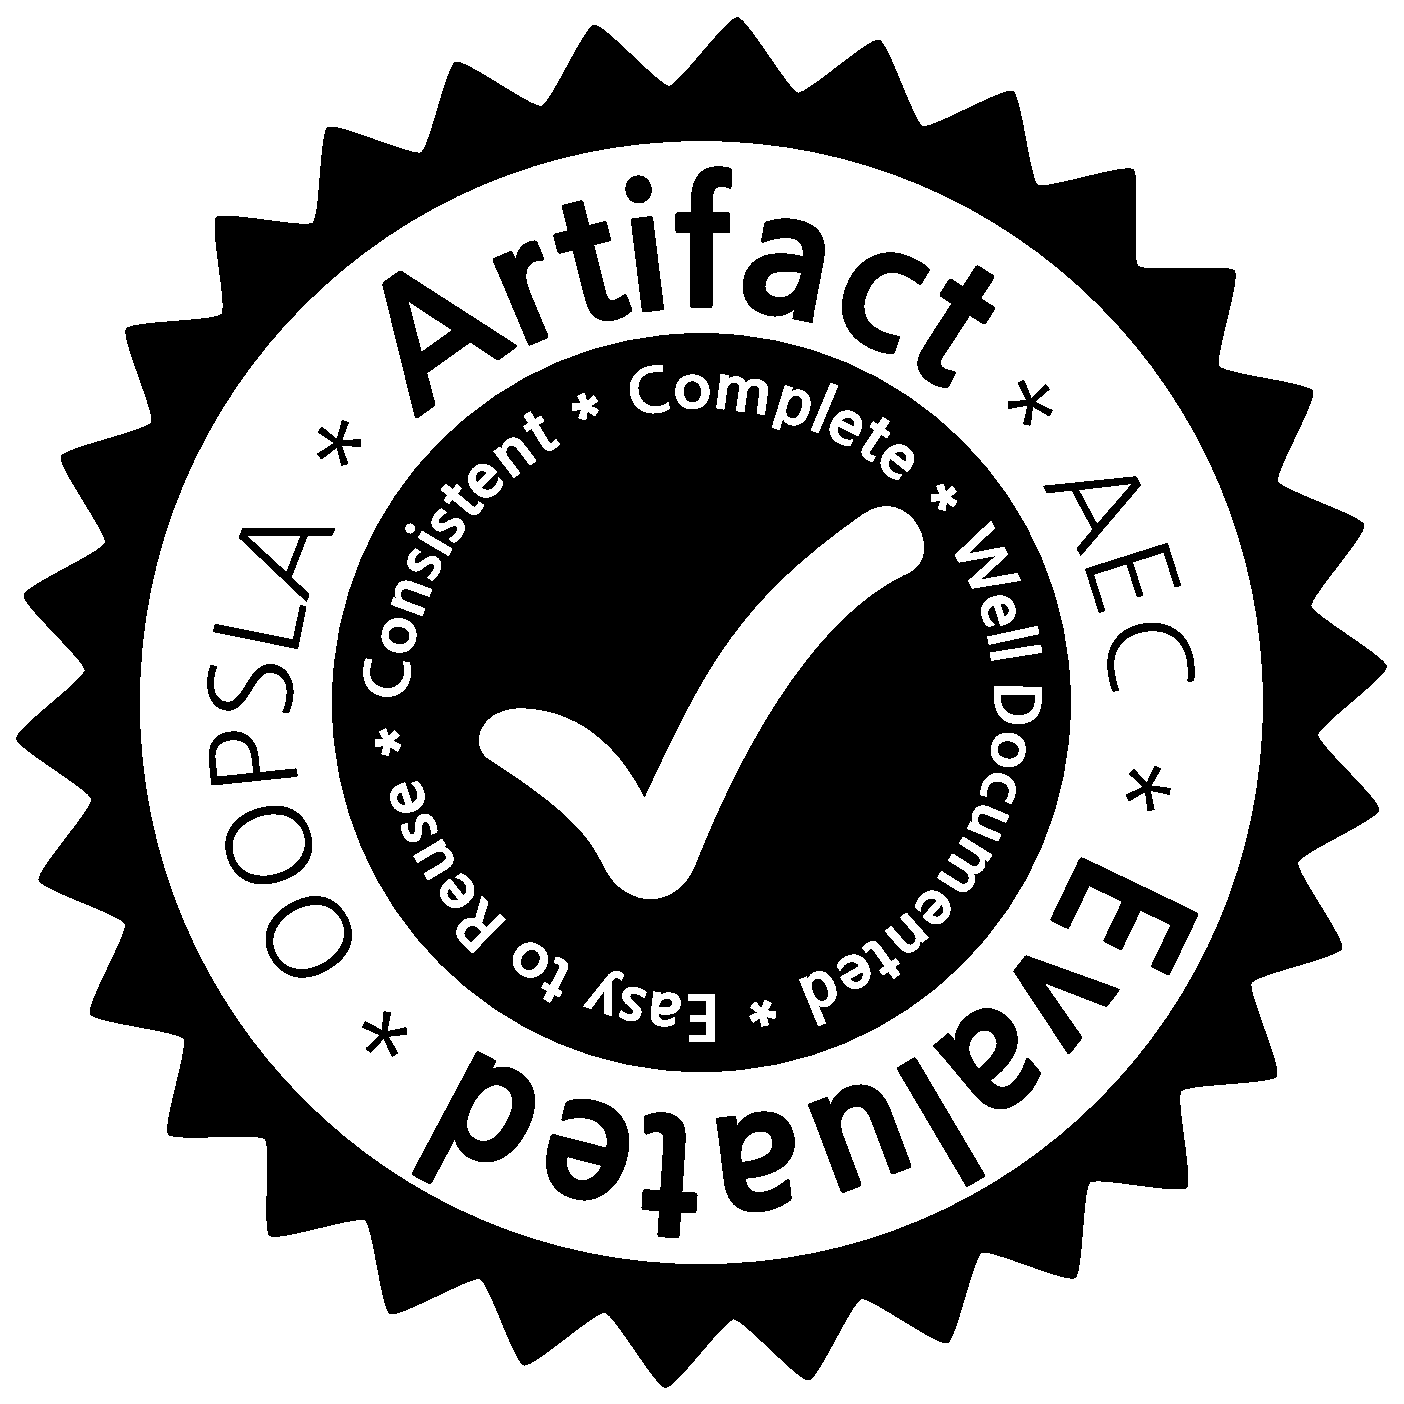
\includegraphics[width=20mm]{aec-badge.eps}
  \vspace{-4em}
\end{wrapfigure}

The papers are used in the thesis with the co-authors' permission.

The implementation artifacts for the first three papers have been checked by the OOPSLA Artifact Evaluation Committee and have received the seal of quality. The PPPJ conference does not offer a similar distinction.
The plugin implementations are openly available: \cite{miniboxing-www,ildl-plugin,ldl-staging-plugin,ldl-value-class-plugin,miniboxing-plugin}.


\textbf{Note to the thesis committee:} Unfortunately, due to a misunderstanding on my side, I had to hand in the final thesis draft much sooner than I expected, so the papers have not yet been fully adapted to integrate well into the thesis. This will be done before the private defense.